

%%%%%%%%%%%%%%%%%%%%%%
\section{Geometry of Level Sets}
%\section{Quantifying Nonconvexity}
\label{sec:QuanNoncon}

\subsection{The Greedy Algorithm}
\label{sec:GreedyAlg}
%%%%%%%%%%%%%%%%%%%%%%

 For a pair of models with network parameters $\theta_i$, $\theta_j$, each with $F_e(\theta)$ below a threshold $L_0$, we aim to efficienly generate paths in the space of weights where the empirical loss along the path remains below the threshold.  These paths are continuous curves belonging to $\Omega_F(\lambda)$--that is, the level sets of the loss function of interest.
  
 We provide a greedy algorith, Dynamic String Sampling, which finds such a path below.

\begin{algorithm}
\caption{Greedy Dynamic String Sampling}\label{euclid}
\begin{algorithmic}[1]
\State $\text{$L_0$} \gets \text{Threshold below which path will be found}$
\State $\text{$\Phi_1$} \gets \text{randomly initialize } $$\theta_1$$ \text{, train } $$\Phi (x_i\;\theta_1)$$ \text{ to $L_0$}$
\State $\text{$\Phi_2$} \gets \text{randomly initialize } $$\theta_2$$ \text{, train } $$\Phi (x_i\;\theta_2)$$ \text{ to $L_0$}$

\State $\text{BeadList} \gets $$(\Phi_1,\Phi_2)$
\State $\text{Depth} \gets 0$ 

\Procedure{FindConnection}{$\Phi_1,\Phi_2$}
\State $\text{$t^*$} \gets \text{t such that } $$\frac{d \gamma(\theta_1, \theta_2, t)}{dt} \bigg|_{t} = 0$$  \text{ OR } $$t = 0.5$$ $
\State $\text{$\Phi_3$} \gets \text{train } $$\Phi(x_i; t^*\theta_1 + (1-t^*)\theta_2)$$ \text{ to $L_0$}$
\State $\text{BeadList} \gets \text{insert}$$(\Phi_3$$\text{, after } $$\Phi_1$$\text{, BeadList)}$
\State $\text{$MaxError_1$} \gets \text{$max_t$}$$(F_e(t\theta_3 + (1-t)\theta_1))$$ $
\State $\text{$MaxError_2$} \gets \text{$max_t$}$$(F_e(t\theta_2 + (1-t)\theta_3))$$ $
\If {$\text{$MaxError_1$} > \text{$L_0$ }} \text{ }\Return \text{ FindConnection}$$(\Phi_1,\Phi_3)$$ $
\EndIf
\If {$\text{$MaxError_2$} > \text{$L_0$ }} \text{ }\Return \text{ FindConnection}$$(\Phi_3,\Phi_2)$$ $
\EndIf
\State $\text{Depth} \gets \text{Depth$+1$}$ 
\EndProcedure
\end{algorithmic}
\end{algorithm}
 
  The algorithm recursively builds a string of models in the space of weights which continuously connect $\theta_i$ to $\theta_j$.  Models are added and trained until the pairwise linearly interpolated loss, i.e. $\rm{max}_t F_e(t\theta_i\ +\ (1-t)\theta_j)$ for $t\in(0,1)$, is below the threshold, $L_0$, for every pair of neighboring models on the string.  We provide a cartoon of the algorithm in \figref{fig:AlgorithmFigure}.
 
 \begin{figure}
\begin{center}
\scalebox{1}{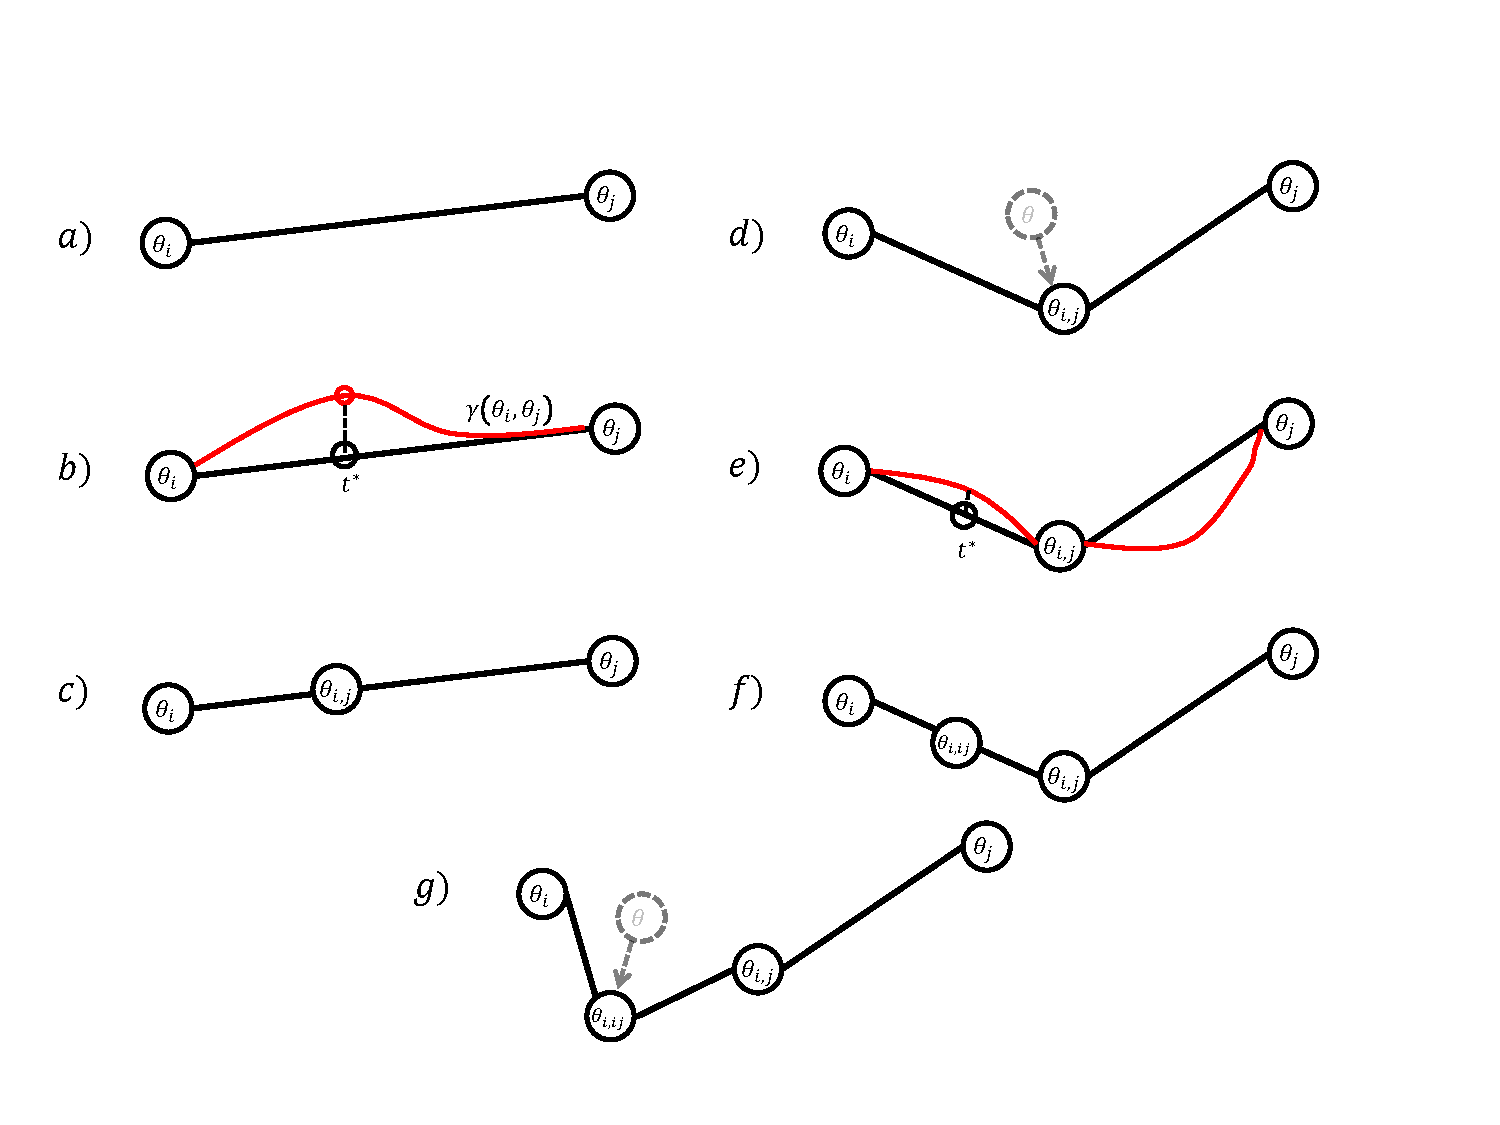
\includegraphics[width=1.0\columnwidth]{../AlgorithmFigure}}
\end{center}
\caption{A cartoon of the algorithm.  $a):$ The initial two models with approximately the same loss, $L_0$. $b):$ The interpolated loss curve, in red, and its global maximum, occuring at $t=t^*$. $c):$ The interpolated model $\Theta(\theta_i, \theta_j, t^*)$ is added and labeled $\theta_{i,j}$.  $d):$ Stochastic gradient descent is performed on the interpolated model until its loss is below $\alpha L_0$. $e):$ New interpolated loss curves are calculated between the models, pairwise on a chain.  $f):$ As in step $c)$, a new model is inserted at the maxima of the interpolated loss curve between $\theta_i$ and $\theta_{i,j}$.  $g):$  As in step $d)$, gradient descent is performed until the model has low enough loss.}
\label{fig:AlgorithmFigure}
\end{figure}
 
  
  \subsection{Failure Conditions and Practicalities}
  \label{sec:Fail}
  
  While the algorithm presented will faithfully certify two models are connected if the algorithm converges, it is worth emphasizing that the algorithm does not guarantee that two models are disconnected if the algorithm fails to converge.  In general, the problem of determining if two models are connected can be made arbitrarily difficult by choice of a particularly pathological geometry for the loss function, so we are constrained to heuristic arguments for determining when to stop running the algorithm.  Thankfully, in practice, loss function geometries for problems of interest are not intractably difficult to explore.  We comment more on diagnosing disconnections more carefully in section SYMMETRYDISCONNECT.
  
  Further, if the $\rm{\mathbf{MaxError}}$ exceeds $L_0$ for every new recursive branch as the algorithm progresses, the worst case runtime scales as $O(\rm{exp}(\rm{\mathbf{Depth}}))$.  Empirically, we find that the number of new models added at each depth does grow, but eventually saturates, and falls for a wide variety of models and architectures, so that the typical runtime is closer to $O(\rm{poly}(\rm{\mathbf{Depth}}))$---at least up until a critical value of $L_0$.  We comment more on this in section NUMERICALDISCUSSION.
  
  Finally, we find that training $\Phi_3$ to $\alpha L_0$ for $\alpha < 1$ in line $8$ of the algorithm tends to aid convergence without noticeably impacting our numerics.
 
